\chapter{Results}

The data clearly show first a relationship between cell state of charge the acoustic TOF through the cell, then between induced lithium plating and changes in acoustic time of flight data, and finally between changes in ambient temperature and change in acoustic TOF through the cell. 

Recall that the three sources of change in acoustic time of flight through a cell are change in state of charge, change in state of health, and change in ambient conditions. 
By systematically adding and understanding changes in each category to the experimental conditions, shifts in acoustic ToF through the cell can be observed, analyzed, and then attributed to each source of change.

SoC and SoH cause changes in the travel time of an ultrasonic signal through the cell due to changes to the cell's bulk properties, including the materials composition of each layer, the stiffnesses and densities of these materials, and the thicknesses of these layers \cite{SOC-SOH-EST}. The relationship between the velocity $V_p$ at which a wave travels through an isotropic elastic material can and the materials properties of the material its traveling through can be expressed as
$$ V_p = \sqrt{\frac{K + \frac{3}{4}G}{\rho}}$$
where $K$ is the material bulk modulus, $G$ is the material shear modulus, and $\rho$ is the material density \cite{SOC-SOH-EST}. This shows that increases in a layer's density will increase the time a wave spends transmitting through a layer, causing a positive TOF shift. Conversely, increases in a layer's bulk and shear moduli (essentially, stiffening of the layer), will allow the ultrasonic wave to propogate through the layer more quickly, causing a negative TOF shift. As the state of charge of the cell changes, lithium ions are forced to move between electrodes, changing the cell's materials composition and materials structure. As the state of health changes, metallic lithium both collects on the surface of the graphite electrode, and fills some of the graphite's pores, changing the stiffness of the material and its density. The density and thickness of various layers of the cell at different states of charge or health is complicated to model, but the particulars aren't actually needed in order to interpret changes in ToF as caused by changes in state of health, state of charge, or even changes in ambient conditions. In order to avoid that complicated analysis, this work focuses on the metric of change in ToF shift. For any given state of health, cycling of state of charge should create a consistently undulating curve, so if a cycle's ToF shift is normalized against the ToF shift data from the first cycle, changes in either state of health or ambient conditions can be observed. The remainder of this paper will step through the analysis to build that up step by step, first by establishing an understanding of the relationship between ToF shift and state of charge, then considering variation in state of health, and finally incorporating change in ambient temperature, a step not taken in prior work.

When this paper discusses wave arrivals, it is shorthand for first-arrival; subsequent arrivals change less straightforwardly than the first arrival since they are impacted by the thickness of each layer and the relative properties of each adjacent layer \cite{SOC-SOH-EST}, complicating analysis without adding much understanding, so are ignored in these analyses.

%%
%% STATE OF CHARGE
%%
\section{Time of Flight Shift Due to Change in State of Charge}
The data clearly demonstrate a strong and consistent relationship between acoustic ToF through the cell and the cell's state of charge while ambient conditions and cell state of health are held steady.  \hyperref[fig:0315]{\cref{fig:0315}} shows a protocol with two C/2.5, two 2C, two 5C, and two 10C charging cycles. The TOF data is very similar for each of the cycles in the C/2.5 and 2C cycles, which would would expect since the temperature is roughly constant, and there should have been no appreciable plating at such gentle cycles. One would expect that if the only cause in ToF shift was change in state of charge, then the ToF at the beginning of the charge cycle and the end of the discharge cycle would be the same, which is approximately the case for the C/2.5 and 2C cycles. Starting a bit with the 5C cycles and becoming quite noticeable with the 10C cycles, there is an offset between the ToF the charging portion of the cycle begins at, and the ToF the discharging portion ends at; this was not the case with the gentle cycles and happens despite the temperature holding relatively steady (about $1^{\circ}$C variation across all four latter cycles), suggesting the cause is lithium plating (a change in the state of health of the cell).

\begin{figure}[t]\label{fig:0315}
    \includegraphics[width=0.55\textwidth]{Thesis/0315.png}
    \centering
    \caption{ToF Shift across the experiment, with load voltage and temperature shift.}
\end{figure}

The shift in ToF was determined using a colleague's cross-correlation analysis of each received waveform to a reference waveform. The reference waveform was chosen from one of earliest waveforms in the experiment, but not too early, in order to allow for start-up effects to dissipate; it was chosen from the initial rest period, before the cell had been introduce to any changes in state of charge or state of health.
During the C/2.5 charge and discharge cycling, which does not appreciably plate the cell and therefore can be assumed to not change the state of health of the cell, the ToF data follows a very regular pattern. 
The ToF shift peaks at roughly the same value, and at the same point in the cycling protocol: when the routine finishes charging. 
Conversely, the ToF shift experiences a minimum of fairly consistent value at the end of each discharge period.

%%
%% STATE OF HEALTH
%%
\section{Time of Flight Shift Due to Change in State of Health}
The data in the same test goes on to demonstrate acoustic ToF analysis's capability to observe plating, and therefore change in a cell's state of health. This is shown during the 5C and especially 10C routines in the experiment. 
While the ToF shift data maintains a consistent form for each of those protocols, the point to which it returns between cycles increases each time. 
Since the ambient conditions were steady and there was no variation in the cycling protocols, these changes in the ToF shift show lingering changes in the state of health of the cell. 
This is corroborated by optical, SEM, and XPS imaging. 
SEM (scanning electron microscope) and XPS (X-Ray Photoelectron Spectroscopy) analyses confirm plating on the electrodes of the cells, but such techniques do not provide information on when the plating occurred.

\begin{figure}[t!]\label{fig:optical}
\centering
     \begin{subfigure}
         \centering
         \includegraphics[width=0.45\textwidth]{optical5c.JPG}
     \end{subfigure}
     \hfill
     \begin{subfigure}
         \centering
         \includegraphics[width=0.45\textwidth]{optical.JPG}
     \end{subfigure}
     \caption{Cells cut open after experiencing 5C and zero (left) or one (center) 10C cycles. The dark regions are the graphite electrode, and the light regions lithiation.}
\end{figure}

Visual analysis provided simple confirmation that the cell had plated; since the cell had not been used before the experimental protocol described above, it can be safely assumed the plating occurred then.

%%
%% SEM ANALYSIS
%%
\subsubsection{SEM Imaging}
\begin{figure}[t!]\label{fig:sem}
\centering
\caption{SEM images of cells after experiencing a few 5C cycles and either zero (left), one (center), or two (right) 10C cycles.}
     \begin{subfigure}
         \centering
         \includegraphics[width=0.3\textwidth]{sem5c.png}
     \end{subfigure}
     \hfill
     \begin{subfigure}
         \centering
         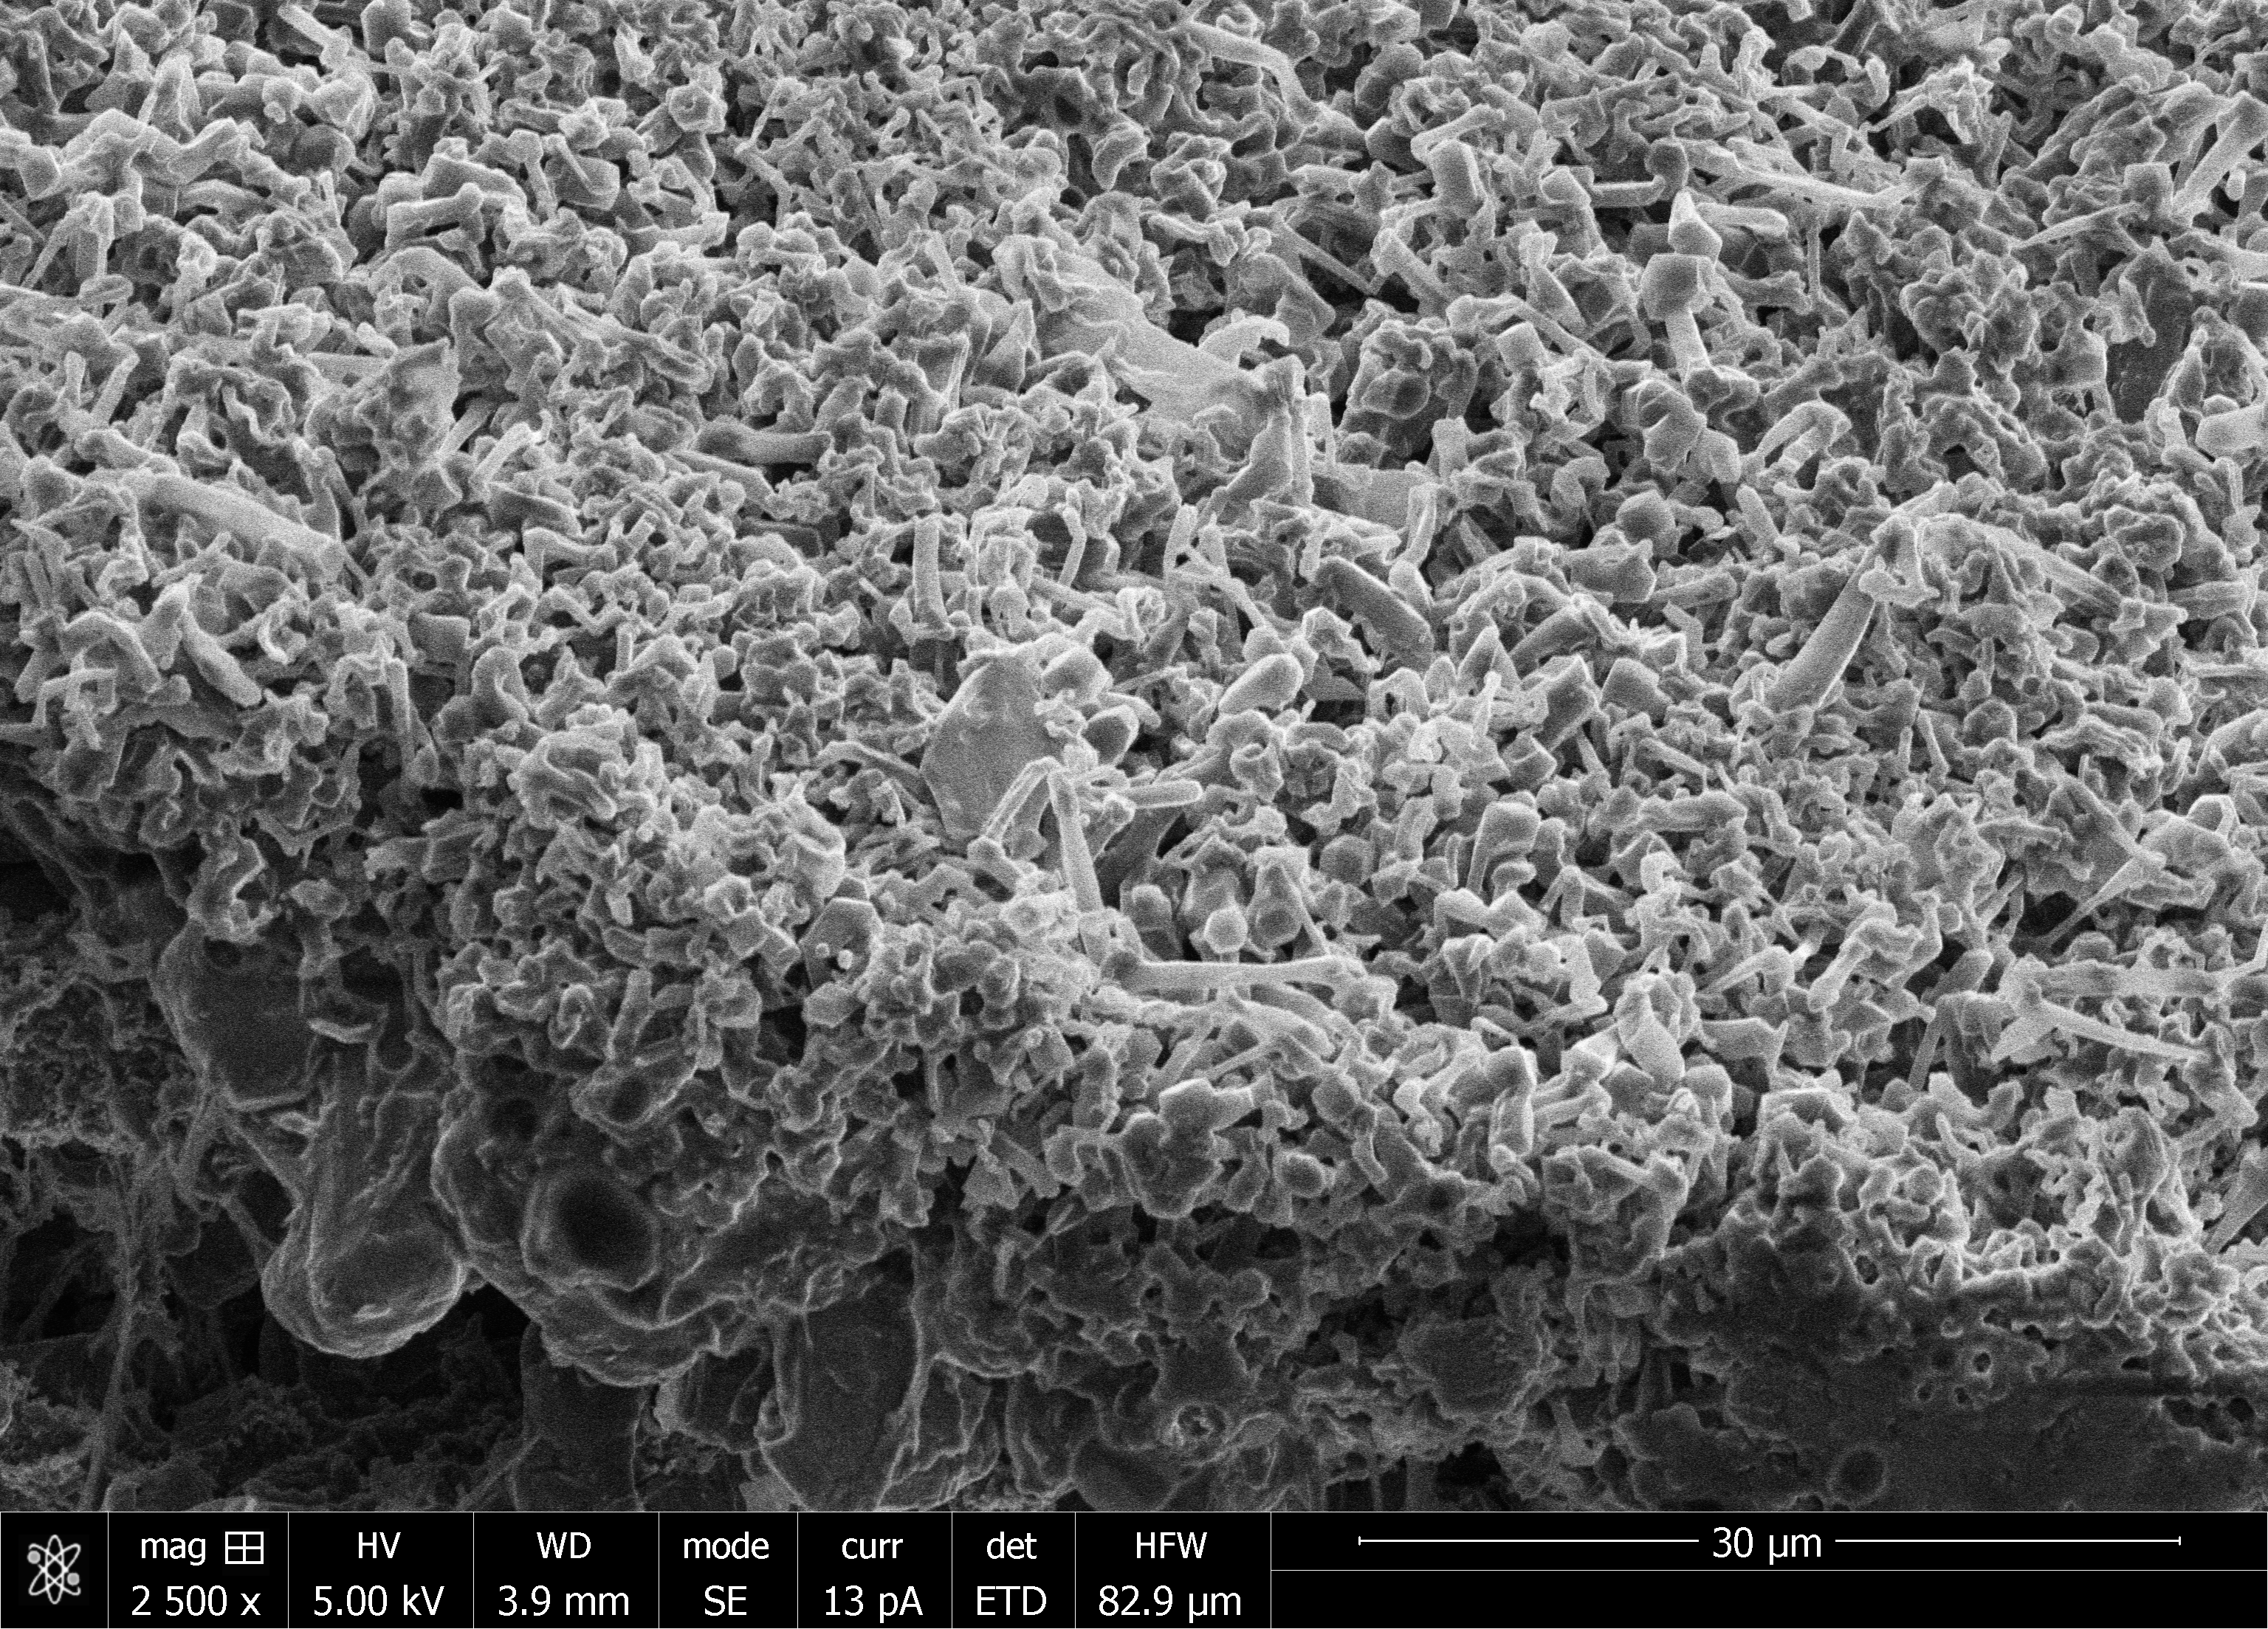
\includegraphics[width=0.3\textwidth]{sem10cx1.png}
     \end{subfigure}
     \hfill
     \begin{subfigure}
         \centering
         \includegraphics[width=0.3\textwidth]{sem10cx2.png}
     \end{subfigure}
\end{figure}

The cells from Experiments A, B, and C were dissected to produce SEM images. Each of these cells had been through a few 5C charge cycles before finishing with either no 10C cycles, one 10C cycle, or two 10C cycles. 

SEM measurements were taken with a Verios 460 XHR with working distance of about 4 mm and accelerating voltage of 5 kV. The cycled graphite anodes were harvested from the cell, rinsed copiously in DMC, and dried in the large antechamber vacuum at 40$^{\circ}$C for 2 hours before transferring to the SEM quick load lock chamber in double sealed containers. The sample preparation was done in an Argon filled glovebox with O$_2 <$ 1 ppm and H$_2$O $<$ 0.3 ppm.

The large bulbous objects are particles of the graphite electrode. The tendrils are lithium plating, which forms in snaking dendrites. 
The more plating, the denser they become, as shown in \hyperref[fig:sem]{\cref{fig:sem}}.  

It was expected based on the ToF shifts that the 5C cycles caused light plating and the 10C cycles each caused heavy plating, and the SEM images confirmed this; see \hyperref[tab:plating]{\cref{tab:plating}}. All three cells show at least some plating, but the amount varies significantly. The cell which experienced no 10C cycles has no contiguous plated surface area, but rather lithium dendrites in some of the graphite's pore spaces. The cells which experienced 10C cycling have significant, continuous layers of plated lithium on the surface of the graphite.

\begin{table}[h]
    \centering
    \begin{tabular}{c|c|c}
         \# 10C Cycles & Estimated Plate Thickness ($\mu$m) & Estimated ToF Shift (ns) \\
         \hline
         0 & $<1$ & 0 \\
         1 & 8.3 & 1.38 \\
         2 & 21.2 & 3.533 \\
    \end{tabular}
    \caption{Comparison of the number of 10C cycles a cell endured and the thickness of its lithium plating.}
    \label{tab:plating}
\end{table}

These measurements have some caveats. 
Firstly, the thickness and density of the plating was not consistent across the whole surface area of the cell, as can be seen in the optical images; this may have been due to pinching around the edges of the cell from its casing.
Secondly, the scissors used to slice part of the cell away for analysis compressed the lithium; how large this effect was, and how consistent, is unknown. 
Thirdly, the plating is interspersed with the electrolyte, so the layer of lithium plating isn't pure lithium but rather a mixture.
Some of the lithium is also interspersed in pores within the graphite mass.

The speed of sound through lithium is 6000 m/s \cite{lithium}. According to the simple relation

$$ distance = rate \times time \rightarrow \frac{distance}{rate} = time$$

the measured change in acoustic ToF attributable to the change in volume due to lithium plating is 1.38ns for the cell that endured one 10C cycle, 3.533ns for the cell that endured two 10C cycles, and an immaterial amount for the cell that endured zero 10C cycles. Clearly, the sheer added distance the wave must traverse due to the thickness of the lithium plating is not the primary driver of change in acoustic ToF due resulting from changes to the cell's state of health. The rough math here assumes discrete layers of electrode, lithiation, and electrolyte, but that is not the case.
It assumes the cell's strenuous operation and resulting lithium plating had no effect on the graphite.
It also assumes a solid lithium plate of constant density, which, to reiterate, is not truly the case. Nonetheless, those should have small effects on the response. 

The literature suggests that volume changes of other components of the cell would have similarly small contributions to the change in acoustic ToF. Siegel et al demonstrated that repeated 5C cycling of lithium ion pouch cells experienced a volume expansion of just 1.5\% across 21 cycles \cite{EXPANSION}, suggesting that the cells in these experiments would have experienced similarly small changes in volume, which would have minimally contributed to the changes in ToF shift following plating. Indeed, Davies et al induced an increase in cell thickness by charging a pouch cell yet found that due to the overwhelimg influence of other factors on ToF, the cell's ToF actually decreased as the cell charged \cite{SOC-SOH-EST}.

That said, it could be argued that the gradually increasing ToF shifts from the 5C and especially 10C cycles are due to viscoelastic relaxation - while the 10 minute rest periods between cycles was enough for the C/2.5 and 2C cycles, the more strenuous cycles perhaps require more time for full relaxation. However, this is refuted by the data from the longer three hours rests which serve as transitions between charging rates. Take as example the three hour rest between the 5C and 10C rates in Experiment D; the ToF shift is near constant, suggesting no relaxation takes place, and the progressively increasing ToF shift during that cycle was in fact due to plating; the optical, SEM, and XPS imaging results reinforce this.

%%
%% XPS ANALYSIS
%%
\subsubsection{XPS Results}
XPS measurements were taken with a ThermoFisher K-Alpha XPS with Al Kα source. The cycled graphite anode was harvested from the cell, rinsed copiously in DMC, and dried in the large antechamber vacuum at 40$^{\circ}$C for 2 hours before transferring to the XPS with a vacuum transfer module. The sample preparation was done in an Argon filled glovebox with O$_2 <$ 1 ppm and H$_2$O $<$ 0.3 ppm. Peak fitting and analysis was done using the Avantage software, with a Shirley background subtraction and 30\% Lorentzian/Gaussian fit. The spot size was 400 $\mu$m.

The cell from Experiment A was analyzed using XPS analysis. Peak fitting of the Li1s scan results in deconvolution to four peaks at binding energies of 57.72 eV, 56.41 eV, 54.96 eV, and 58.48 eV. Those peaks suggest the presence of metallic lithium, which Wood and Teeter found to have a binding energy of 54.97 eV \cite{BE}. Metallic lithium ought not be present during nominal operation of a lithium-ion cell but will deposit as a result of strenuous cycling \cite{lithium}. Therefore, the XPS data corroborates the results of the above proposed interpretation of the acoustic ToF analysis, as well as the optical and SEM imaging.

\begin{figure}[h!]\label{fig:xps}
    \includegraphics[width=0.85\textwidth]{Thesis/xps.png}
    \centering
    \caption{Li1s scan results from XPS imaging of the cell from Experiment A.}
\end{figure}

%%
%% TEMPERATURE STUFF
%%
\section{Time of Flight Shift Due to Change in Ambient Conditions}
When the ambient conditions were steady, the relationship between SoC and ToF was very clear, as shown in \hyperref[fig:0315]{\cref{fig:0315}}. Ambient temperature variation clearly has a significant effect on the acoustic TOF shifts. \hyperref[fig:adj]{\cref{fig:adj}} shows a comparison between the measured TOF data and "idealized" TOF from a gentle, non-plating routine, constructed by assuming the data ought not change between cycles and copying the first waveform repeatedly as a result. In the absence of plating and at the same state of charge, the relationship between change in ToF shift and change in ambient temperature is consistent enough that much of the influence of temperature can be scrubbed out using simple regressions.

In the first experiment which demonstrated the technique, ambient temperature was held quite steady, and had no material impact on acoustic TOF through the cell. 
However, subsequent experiments were unable to maintain such optimal conditions.
During routines using gentle C/2.5 cycling, thus maintaining state of health, the influence of ambient temperature changes on acoustic TOF can be isolated from the influence of state of charge changes with reasonable success. 
Polynomial fits and linear regressions correlate change in ambient temperature with change in ToF shift. 

The thermocouples and transducers have different sampling rates and schedules, so a couple approaches created paired change in ToF shift and change in temperature data; these are compared in \hyperref[fig:0417temp]{\cref{fig:0417temp}}. 
In one version of the analysis, change in temperature data was averaged across a cycle and regressed against change in TOF shift data. 
\begin{figure}[t]\label{fig:0417temp}
    \includegraphics[width=0.55\textwidth]{0417temp.png}
    \centering
    \caption{Calculated vs measured temperatures.}
\end{figure}
More accurate results resulted from interpolating the temperature data using linear or polynomial fits, depending on the shape of the temperature data.

The analysis shows a reasonable estimate at how the ToF would shift without the influence of the ambient temperature shifts, potentially broadening the application of the technique in monitoring cells. The data from Experiment D provides the following correction to remove the influence of temperature fluctuations from time of flight data:
$$ \text{ToF}_{adj} = \text{ToF}_{meas} + 33.46\Delta T^2 + 48.35\Delta T + 13.41)$$

\begin{figure}[t!]\label{fig:adj}
\centering
     \begin{subfigure}
         \centering
         \includegraphics[width=0.48\textwidth]{Thesis/0409adj.png}
     \end{subfigure}
     \hfill
     \begin{subfigure}
         \centering
         \includegraphics[width=0.48\textwidth]{Thesis/0417adj.png}
     \end{subfigure}
     \caption{ToF shift across experiment duration. These compare the unaltered ToF shift, the ToF shift adjusted using a change in ToF - $\Delta T$ regression using interpolated temperatures, and the ToF shift adjusted using a regression of maximum change in ToF shifts and averaged $\Delta T$ (D only). The horizontal lines represent the baseline ToF shift that, in ideal conditions, would occur during the intercycle rest.}
\end{figure}

Visually, these adjustments are reasonably accurate. 
One check is to compare them to an idealized prediction of how the TOF should actually shift during the experiment. 
Since each cycle at a particular charge rate has a consistent duration and consistent effect on the cell's state of charge, it is easy to compare ToF shift data between cycles. 
At any particular point in the cycle's duration, the ToF shift in each cycle should match. Charge and discharge cycle ToF data, when overlaid (see \hyperref[fig:0417overlays]{\cref{fig:0417overlays}}), show how consistent or inconsistent the ToF shifts are across the experiment.
Ideally there would be perfect overlap in the data from each cycle within a protocol within an experiment, but before the ambient temperature shift's influence was removed, this was clearly not the case. 
The overlap is still imperfect after the TOF shift data was adjusted based on the regressions, but it is much better.

\begin{figure}[t]\label{fig:0417overlays}
\includegraphics[width=0.95\textwidth]{Thesis/0417overlays.png}
\centering
\caption{Overlays of the raw and adjusted ToF shifts across each charge cycle (far and center left) and discharge cycle (center and far right) from Experiment D. The adjusted data used a regression to remove the influence of ambient temperature fluctuations.}
\end{figure}

\begin{figure}[t]\label{fig:0409overlays}
\includegraphics[width=0.95\textwidth]{Thesis/0409overlays.png}
\centering
\caption{Overlays of the raw and adjusted ToF shifts across each charge cycle (far and center left) and discharge cycle (center and far right) from Experiment C. The adjusted data used a regression to remove the influence of ambient temperature fluctuations.}
\end{figure}
